\chapter{Large Language Models}
\label{cap:large_language_models}

% TODO:daniel: Hacer capítulo de Large Language Models

\section{Historia de los Large Language Models}
\label{sec:historia}

El lenguaje es una de las habilidades más importantes que tenemos los seres humanos, y es
que gracias a esta habilidad podemos comunicarnos entre nosotros. Pero, las maquinas no
tienen esta habilidad, a menos que las equipemos on algoritmos poderosos de inteligencia
artificial. Pero aun así siempre a sido un reto conseguir que las maquinas puedan leer, 
escribir y comunicarse como los humanos.

\begin{figure}[H]
    \begin{center}
      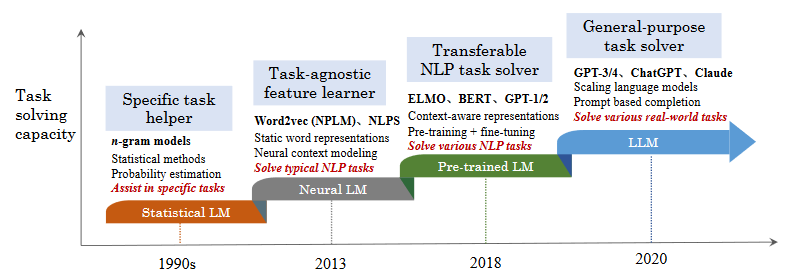
\includegraphics[width=15cm]{figuras/Capitulo_09/EvolutionLM.png}
    \end{center}
    \caption[Proceso de evolución de las cuatro generaciones de modelos lingüísticos (LM) desde la perspectiva de la capacidad de resolución de tareas.]{Proceso de evolución de las cuatro generaciones de modelos lingüísticos (LM) desde la perspectiva de la capacidad de resolución de tareas.(\cite{ZhaoWayneXin2023ASoL})}
    \label{fig:evolutionLM}
\end{figure}\

\textit{Lenguage modeling} (LM) es, a dia de hoy, una de las mejores aproximaciones para conseguir
que las maquinas puedan entender el lenguage humano. La investigación en LM se puede dividir
en cuatro etapas \cite{ZhaoWayneXin2023ASoL}:

% TODO:daniel: Revisar la traducción de este párrafo

\begin{enumerate}
    \item \textit{Statistical language models (SLM)}: Estos modelos estan desarrollados basados en aprendizaje
        estadiístico, y se basan en la probabilidad de que una secuencia de palabras aparezca en un texto. Los 
        SLM se ha aplicado ampliamente para mejorar el rendimeitno de las tareas de recuperación de información
        y el procesamiento del lenguaje natural. Sin embargo, los SLM tienen una gran limitación, es díficil
        estimar con precisión modelos lingüísticos de alto orden exponencial de probabilidades de transición.
    \item \textit{Neural language models (NLM)}: Los NLM se basan en redes neuronales para estimar la probabilidad
        de una secuencia de palabras. Los NLM han demostrado ser más efectivos que los SLM, pero tienen una gran
        limitación, y es que se necesitan grandes cantidades de datos de entrenamiento para poder obtener buenos
        resultados.
    \item \textit{Pre-trained language models (PLM)}: Los PLM son modelos lingüísticos preentrenados que se pueden
        utilizar para resolver tareas de procesamiento de lenguaje natural. Los PLM se entrenan en grandes conjuntos
        de datos de texto sin etiquetar, y se pueden utilizar para resolver tareas de procesamiento de lenguaje
        natural (NLP) específicas con un ajuste fino. Los PLM han demostrado ser muy efectivos en una amplia gama
        de tareas de NLP, pero tienen una gran limitación, y es que se necesitan grandes cantidades de datos de
        entrenamiento para poder obtener buenos resultados.
    \item \textit{Large language models (LLM)}: Los LLM son modelos lingüísticos que se entrenan en grandes conjuntos
        de datos de texto sin etiquetar y se pueden utilizar para resolver tareas de NLP específicas con un ajuste
        fino. Los LLM han demostrado ser muy efectivos en una amplia gama de tareas de NLP, y se pueden entrenar
        con conjuntos de datos de entrenamiento más pequeños que los PLM.
\end{enumerate}

En mi caso, haremos incapie en los LLM, ya que son los modelos que se han utilizado para la realización de este
proyecto. Tipicamente los \textit{Large Language Models} se refiere a modelos de lenguajes que 
tienen cientos de billones de parámetros, y que son entrenados con datos masivos de texto.
Algunos de estos modelos son GPT-3, PaLM, Galactica o LLaMA. Estos modelos han demostrado altas
capacidades para entender el lenguaje natural y resolver tareas complejas a traves del lenguaje o texto.

Así mismo, dentro de los LLM estos han hido creciendo en tamaño y en cantidad de parámetros.
Para ilustralo, en la figura \ref{fig:evolutionLLM} podemos ver la evolución de los LLM a lo largo

\begin{figure}[H]
    \begin{center}
      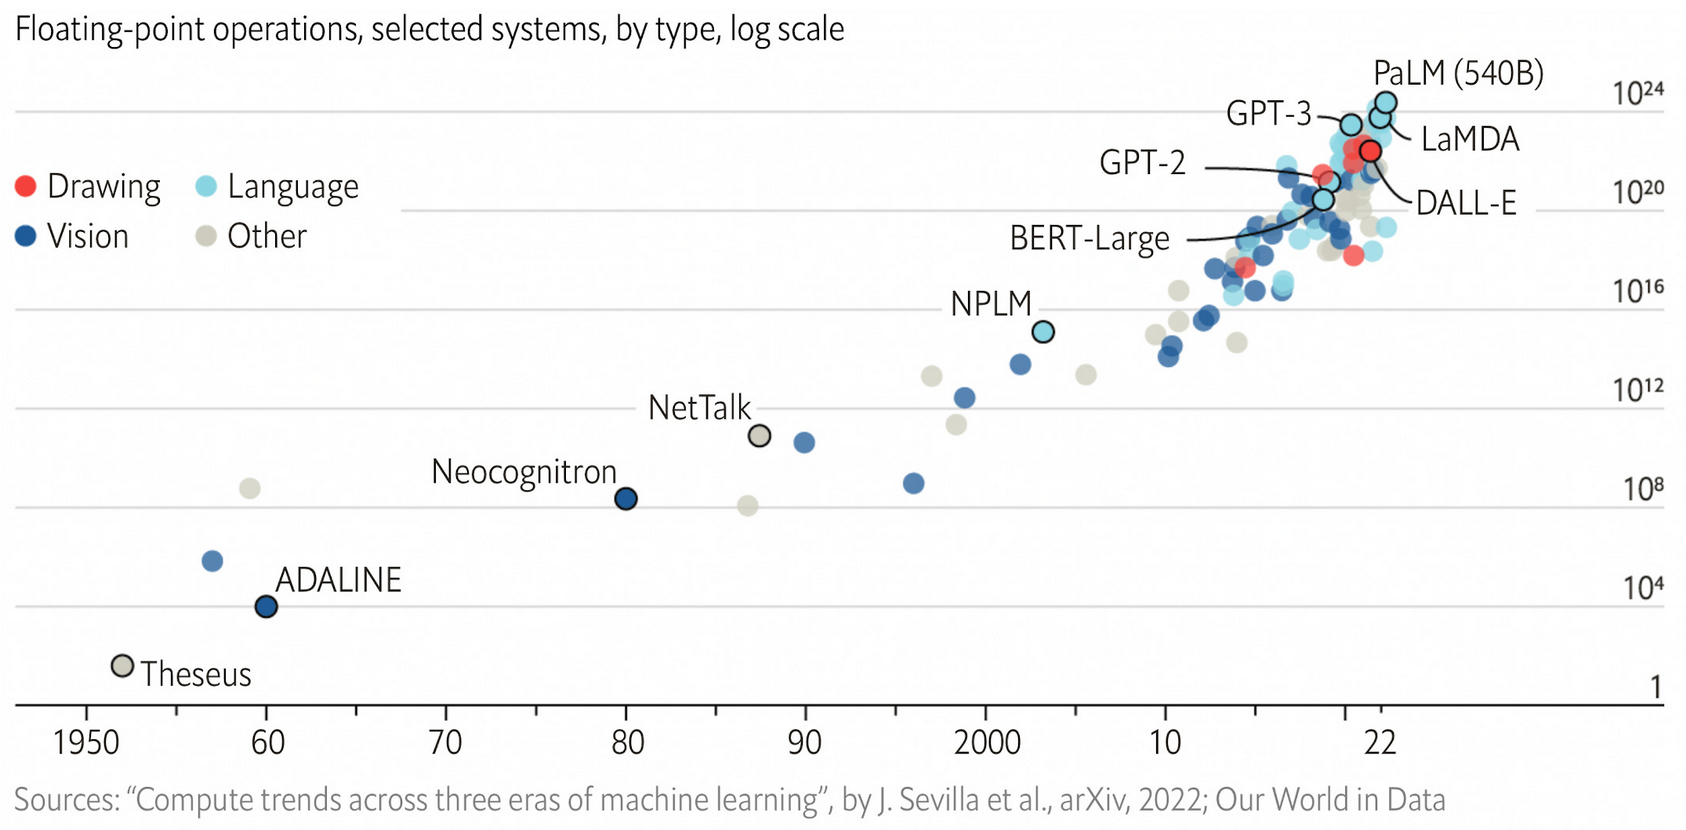
\includegraphics[width=15cm]{figuras/Capitulo_09/EvolutionLLM.png}
    \end{center}
    \caption[Operaciones de coma flotante por tipo en escala logarítmica]{Operaciones de coma flotante por tipo en escala logarítmica (\cite{EvolutionLLM})}
    \label{fig:evolutionLLM}
\end{figure}\

Pero lo que hace realmente interesante estos tipos de modelos es el concepto de
\textit{emergent abilities}, que nos viene a decir que hay abilidades que en 
modelos pequeños no se observan pero que en modelos grandes aparecen. Tres
habilidades que se han observado en los modelos grandes son:

\begin{itemize}
    \item \textbf{\textit{In-context learning}:} esta habilidad es la capacidad
        de generar el texto correcto a partir de una o mas instrucciones en texto
        natural mas un conjunto de demostraciones de como se debe realizar la tarea.
        El modelo es capaz de realizar la tarea sin necesidad de entrenamiento previo.
        Esta habilidad fue introducida formalmente por GPT-3.
    \item \textbf{\textit{Instruction following}:} esta es la habilidad de seguir
        instrucciones por las cuales no se a entrenado, es decir, si hacemos un 
        \textit{fine-tuning} de un modelo con un conjunto de multitareas formateadas en
        lenguaje natural, el modelo es capaz de realizar las tareas sin necesidad de
        entrenamiento previo.
    \item \textbf{\textit{Step-by-Step reasoning}:} esta es la habilidad de resolver
        problemas de razonamiento complejos, concretamente en resolver tareas que
        requieren de multiples pasos de razonamiento.
\end{itemize}

\section{Fine-tuning}
\label{sec:fine_tuning}

El fine-tuning o en castellano ''ajuste fino'' es una técnica en la cual podemos ajustar 
ciertos pesos en las camas de nuestra red neuronal, este ajuste lo podremos hacer para 
todas las capas o solo para un subconjunto de ella. Esta técnica se utiliza para poder
adaptar un modelo preentrenado a una tarea especifica.

\begin{figure}[H]
    \begin{center}
      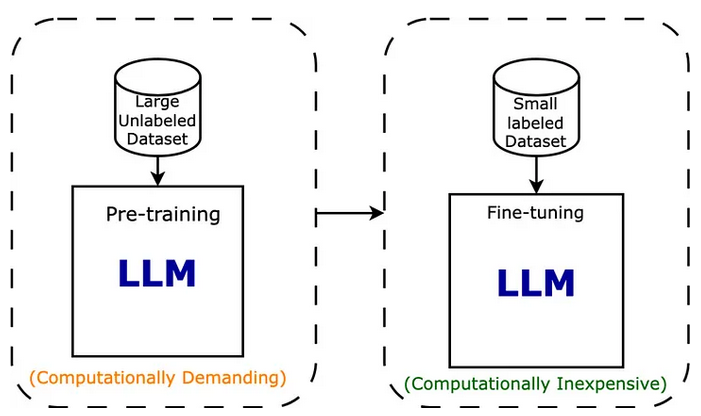
\includegraphics[width=15cm]{figuras/Capitulo_09/TrainVSFinetuning.png}
    \end{center}
    \caption[]{(\cite{SupervisedFineTuning})}
    \label{fig:finetuning}
\end{figure}\

\begin{figure}[H]
    \begin{center}
      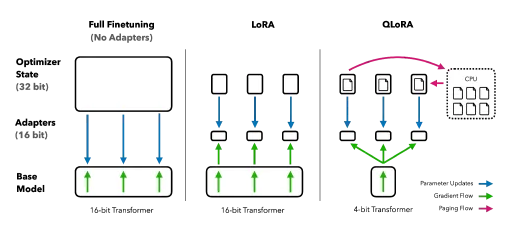
\includegraphics[width=15cm]{figuras/Capitulo_09/QLoRa.png}
    \end{center}
    \caption[]{(\cite{SupervisedFineTuning})}
    \label{fig:qlora}
\end{figure}\
